\documentclass{article}
\usepackage[T1]{fontenc}
\usepackage{lmodern}
\usepackage{graphicx}
\usepackage{amsmath,amssymb}
\usepackage[a4paper,margin=2cm]{geometry}
\usepackage[absolute,overlay]{textpos}
\setlength{\TPHorizModule}{1mm}
\setlength{\TPVertModule}{1mm}
\usepackage[indonesian]{babel}
\usepackage{hyperref}
\setlength{\emergencystretch}{2em}
% unit: Halaman 28

\begin{document}

% === Halaman 28 (llm) ===

\vspace{243.54mm}

Demo Online RSA 3: \url{https://www.lddgo.net/en/encrypt/rsa}

% deskripsi: Screenshot antarmuka situs web RSA Encryption and Decryption Online yang menunjukkan kolom Input Content, Input Key, dan berbagai opsi pengaturan enkripsi seperti Mode (ECB), Padding (PKCS1Padding), dan Key Type (Private Key).
% bbox normalisasi: [0.0400, 0.1400, 0.9500, 0.9600]
\begin{textblock*}{191.10mm}(8.40mm,41.58mm)
\noindent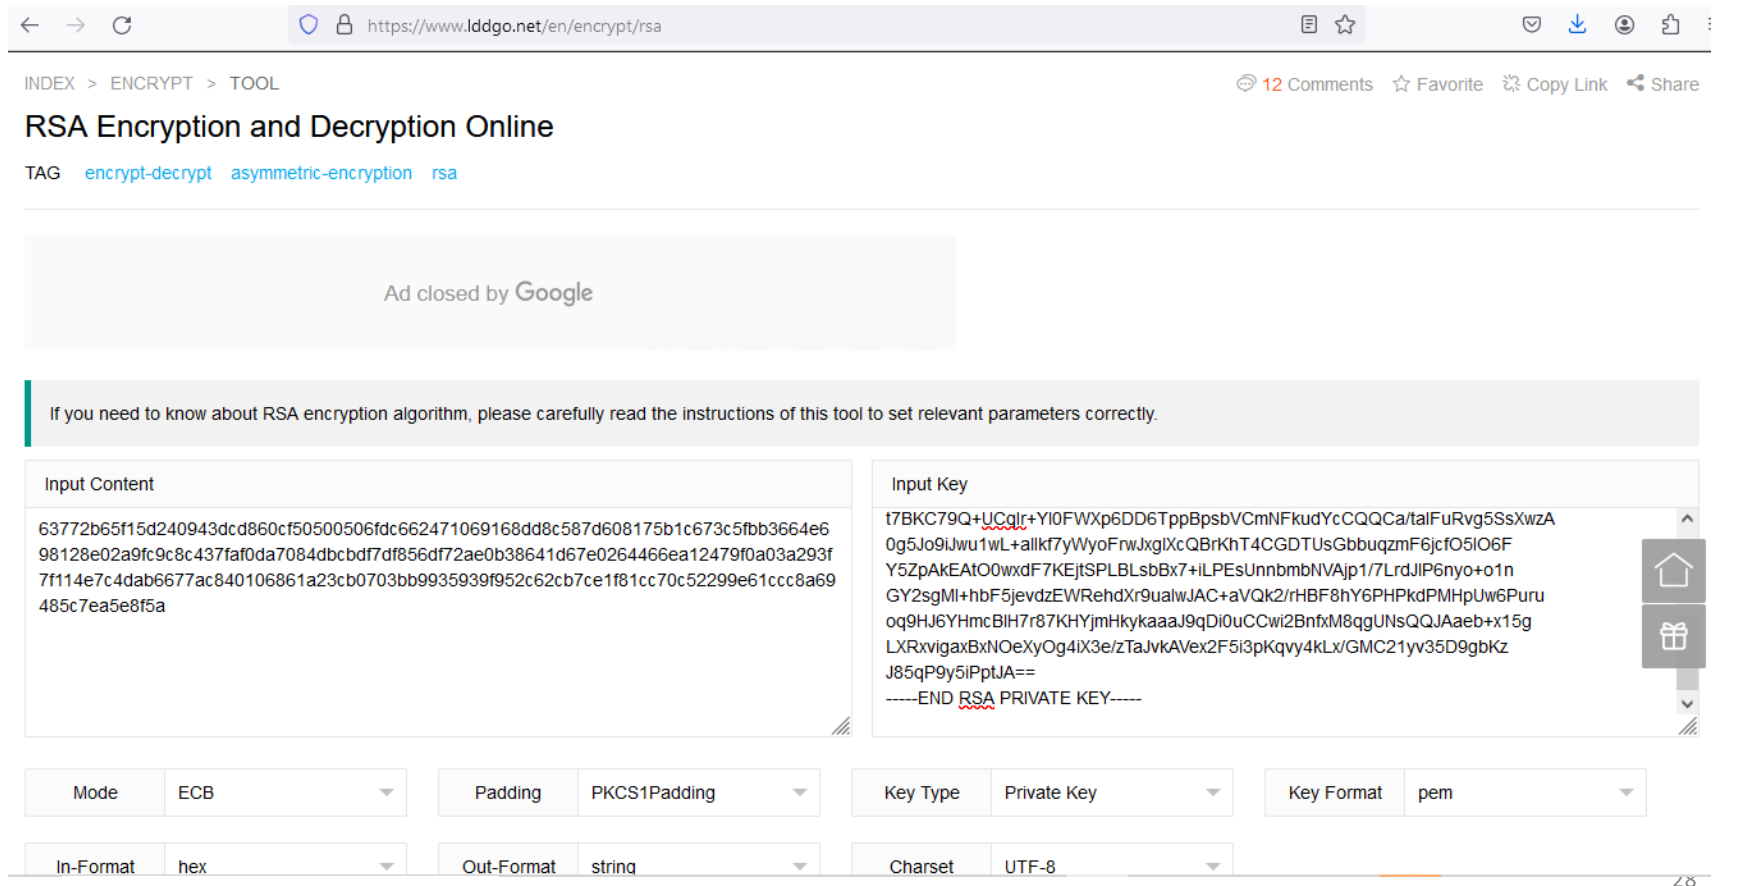
\includegraphics[width=191.10mm,height=243.54mm]{../../images/llm/page_028_img_01.png}%
\end{textblock*}

\end{document}
